\chapter{Applications}
\label{chap:apps}

As mentioned in previous chapters, the SSaaS model can be utilized
across a range of existing and proposed applications. In each case,
the model allows users to reduce the trust they must place in any
single third party while retaining support for popular use cases
today. I present several potential SSaaS applications in this chapter.

\section{Storage}

One of the primary applications of the SSaaS model is to secure
storage systems, both local and hosted. These applications are all
variations on the previously discussed encrypted data + SSaaS-backed
keys model. In such applications, users handle the encrypting and
decryption of data locally, only sending encrypted data to third
parities or storing it on high risk devices. In order to ensure that
such client-side encryption does not break traditional features
associated with cloud and mobile data storage, clients store the
associated encryption keys with one or more Secret Storage Providers.

\subsection{Cloud File Sync/Storage}

\begin{figure}[t]
  \centering
  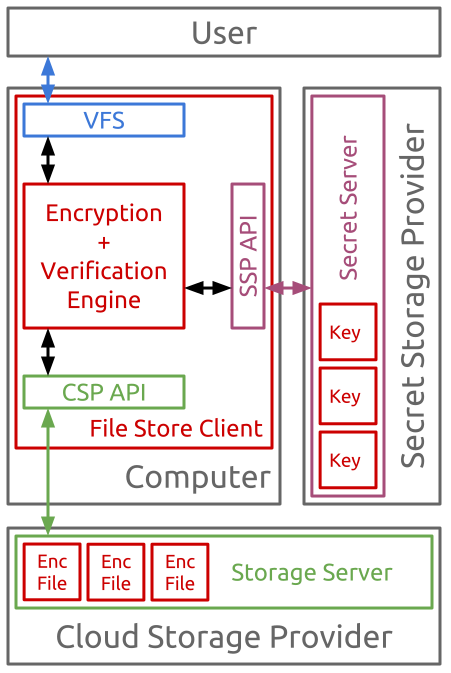
\includegraphics[width=150px]{./figs/out/App-FileStore.pdf}
  \caption{SSaaS-Backed Cloud File Storage System}
  \label{fig:apps-filestore}
\end{figure}

Building on the original motivating example in this proposal, using
Dropbox without trusting Dropbox with plain-text user data, we can
construct an SSaaS-backed cloud sync and storage
client. Figure~\ref{fig:apps-filestore} illustrates this
application. As in the general storage case, this applications
involves applying client-side encryption/decryption (e.g. using
AES~\cite{nist2001}) and authentication/verification (e.g. using
CMAC~\cite{dworkin2005}) on every read and write to a third-party
backed data store. The third-party data store holds only encrypted and
authenticated data, ensuring that the third party need not be provided
with the Access (\emph{R}-type) and Manipulation (\emph{W}-type)
capabilities.

In order to ensure that users can still share data with other users
and sync it across devices, all required encryption and authentication
keys are stored with one or more SSPs. When a user wishes to sync data
to a new device, they grant said device access to the necessary keys
via their SSP's management interface. The new device can then download
the encrypted files from the minimally trusted storage provider and
decrypt/verify them using the keys provided by the SSP. Device
authentication can be provided via certificates, shared-secrets
(e.g. passwords), or contextual information as proposed in
Chapter~\ref{chap:custos}. When a user wishes to share data with
another user, they grant the new user access to data via the storage
providers normal sharing mechanisms. They then also grant the new user
access to the necessary keys via the SSPs management mechanisms. The
user can now download the data from the storage provider and decrypt
and verify it with the keys form the SSP. As in the syncing case,
authentication may be performed via a variety of mechanisms, allowing
the data owner to select the authentication primitives best suited for
a given situation.

This type of applications thus overcomes the traditional deficiencies
of secure cloud-based data storage. It minimizes trust in the third
party storage provider by only granting them access to encrypted and
authenticated data. But it also maintains support for the multi-device
and multi-user use cases traditionally associated with cloud-backed
data storage. The SSaaS model allows users to enhance their privacy
and security by reducing exposure to third parties without incurring
undue additional usability burdens or denying access to desirable use
cases.

\subsection{Server Full Disk Encryption}

\subsection{Mobile Device Encryption}

\section{Communication}



\section{Authentication}

\subsection{Managed SSH}


%%  LocalWords:  SSaaS CMAC SSPs SSP's SSP
